
\documentclass[11pt]{article}
\usepackage[letterpaper, margin=1in]{geometry}

% Used to place appendix in the toc with proper titles
\usepackage[toc,page,title]{appendix}
\renewcommand{\appendixname}{Appendix} % Used to rename from "Appendices" to "Appendix"
\renewcommand{\appendixpagename}{Appendix} % Used to rename from "Appendices" to "Appendix"
\renewcommand{\appendixtocname}{Appendix} % Used to rename from "Appendices" to "Appendix"

% Used to make citations/bibliography
% Usage:
% \bibliography{./bibliography/fullbib.bib}
% \bibliographystyle{plain}
\usepackage{cite}

% To enable forcing figure placement
\usepackage{float}

% Used to skip to next paragraph when a blank line is used between sentences
\usepackage{parskip}

% Used to change line spacing (double spaced, 1.5, etc.)
% Usage: 
% \begin{spacing}{1.5}
% \end{spacing}
\usepackage{setspace}

% Used for inserting images.
% Usage: 
% \begin{figure}[hpt]
%     \centering
%     \caption{Caption}
%     \includegraphics[width=0.6\textwidth]{images/<IMG.NAME>}
%     \label{fig:<LABEL>}
% \end{figure}
\usepackage{graphicx}
\graphicspath{ {./images/} }

% Subplots
\usepackage{subcaption}

% Used for in text code with formatting and language highlighting
\usepackage{listings}
\usepackage{xcolor}

\usepackage[breaklinks]{hyperref}
\usepackage{url}

% Define custom style
\lstdefinestyle{mystyle}{
    basicstyle=\ttfamily\footnotesize, % Use a monospaced font with strict sizing
    numbers=left, % Show line numbers
    numbersep=5pt,
    numberstyle=\tiny\color{gray},
    stepnumber=1, % Ensures every line gets numbered
    tabsize=4, % Set tab width
    keepspaces=true, % Preserve spaces
    showspaces=false,
    showstringspaces=false,
    breaklines=true,
    breakatwhitespace=false,
    columns=fixed, % Maintain strict spacing
    lineskip=-1pt, % Prevent additional spacing between lines
    frame=single, % Optional: adds a border around the code
    rulecolor=\color{black},
    backgroundcolor=\color{white},
    keywordstyle=\color{blue}\bfseries, % Style for keywords
    stringstyle=\color{red}, % Style for strings
    commentstyle=\color{gray}, % Style for comments
    xleftmargin=5pt, % Adjusts left margin outside the frame
    xrightmargin=5pt % Adjusts right margin outside the frame
}
\renewcommand{\lstlistingname}{Code Block}


\lstset{style=mystyle}

% Used to create hyperlink references that can be clicked within the PDF
% Usage: \ref{<SECTIONLABEL>}
\usepackage{hyperref}

% Used for certain math symbols
\usepackage{amssymb}

\usepackage{array}
\usepackage{ragged2e}

\usepackage{titlesec}
\usepackage{bookmark}

\setlength\parindent{0pt}

\title{%
  ELEC 873 \\
Assignment 2}

\author{Anthony Sicoie (20214793)}

\begin{document}

\maketitle

\section*{Preamble}

For each question code was developed locally and tested on both my machine (Ryzen 9 7950x, 64 GB Ram) as well as the KNL server.
This is the Makefile template that all questions also followed, with appropriate changes based on the question requirements for each one; where questions only required a single implementation (only OpenMP etc.), only that implementation was accounted for in.
Furthermore, the Makefile was also used to run the code in all cases other than those utilizing bash scripts; in those cases it is mentioned explicitly.
Comments are provided throughout the Code Blocks for any noteworthy or special conditions I felt were worth highlighting.
As such discussion of code within the report is minimal, but rather the comments are intended to describe how the code functions.


\section*{Q1:}

\begin{figure}[H]
\centering
    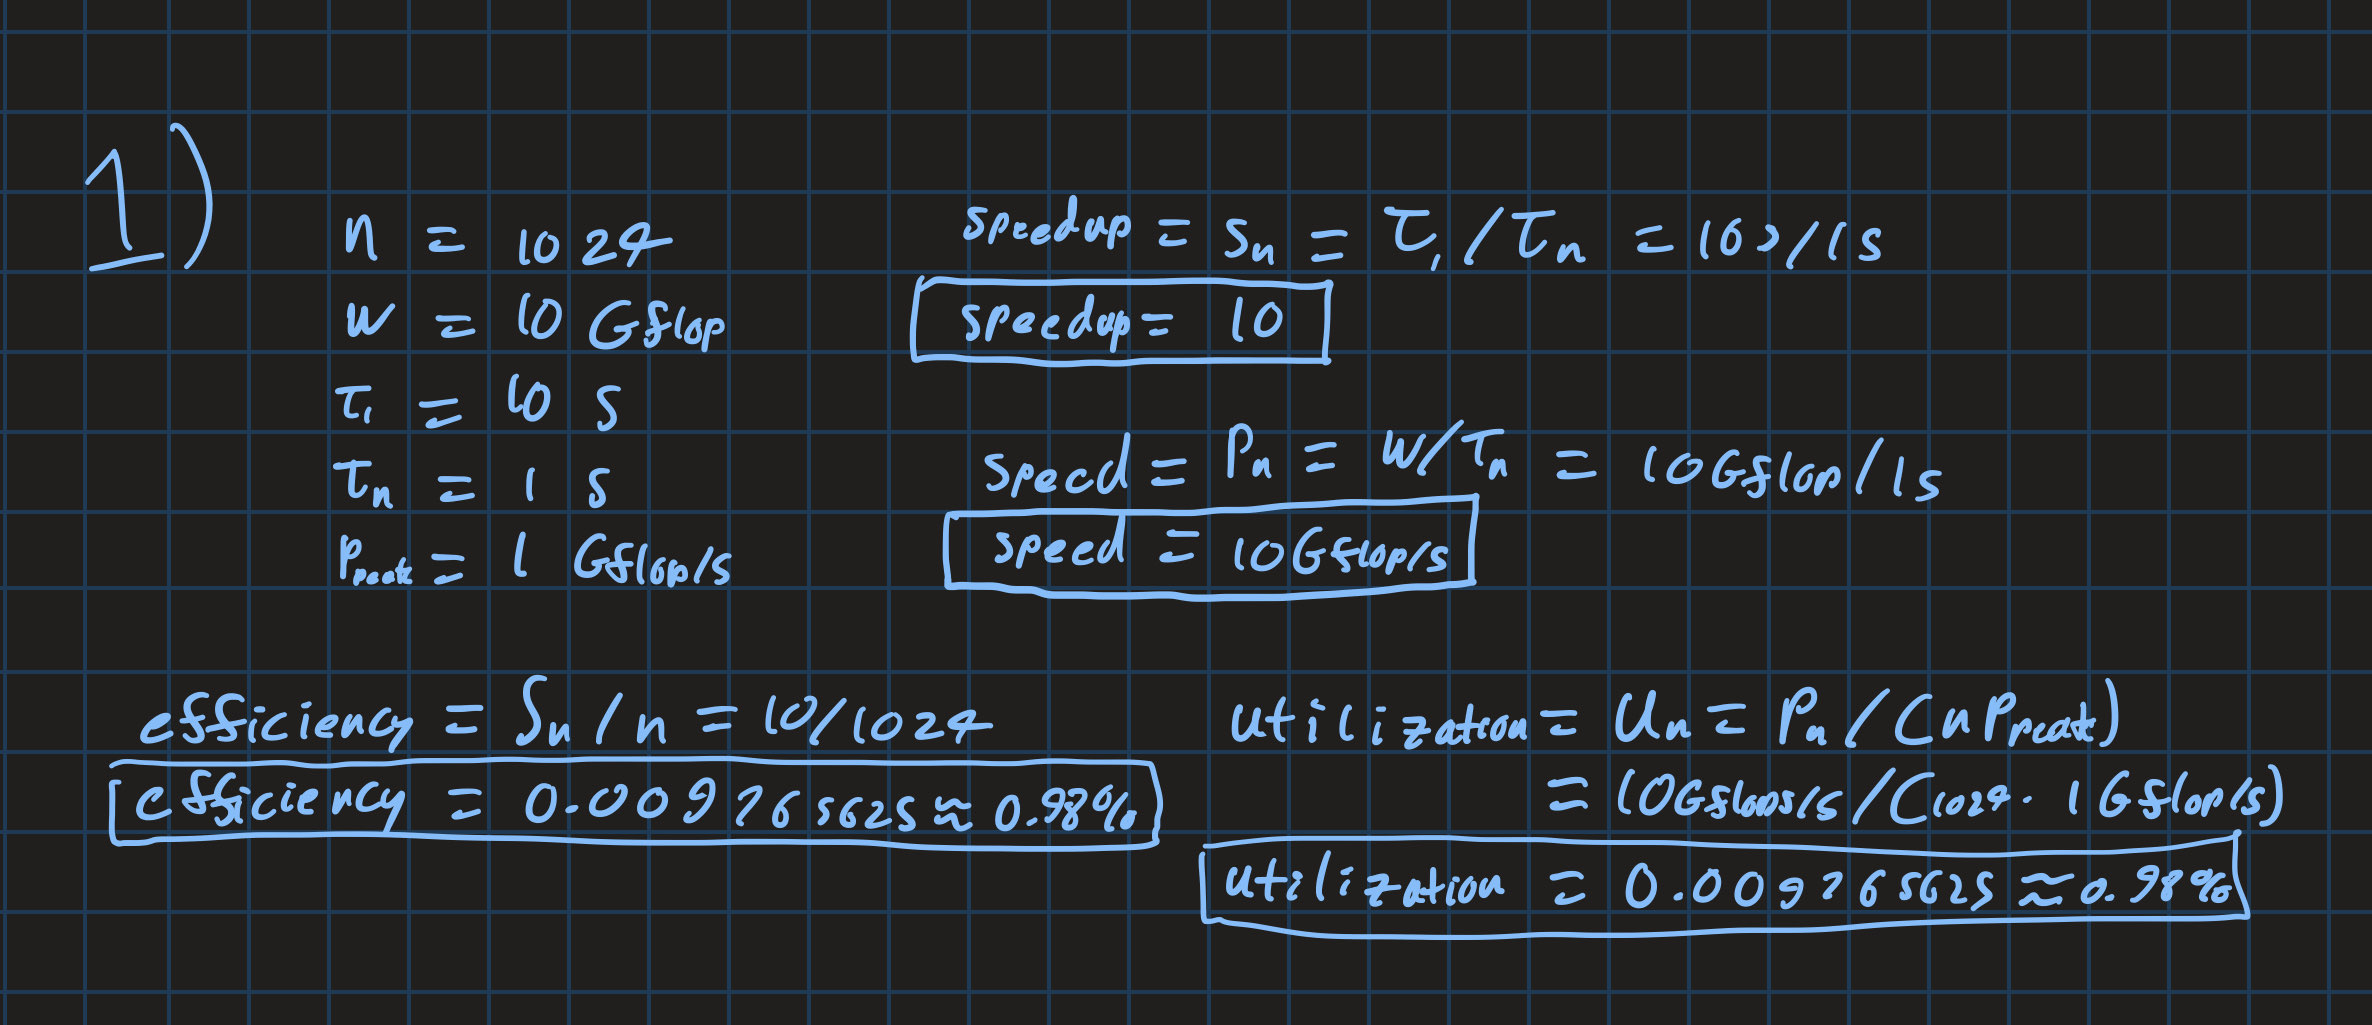
\includegraphics[width=0.9\textwidth]{./images/q1.jpg}
\caption{Math for Question 1}
\label{fig:q1}
\end{figure}

\newpage

\section*{Q2:}

\begin{figure}[H]
\centering
    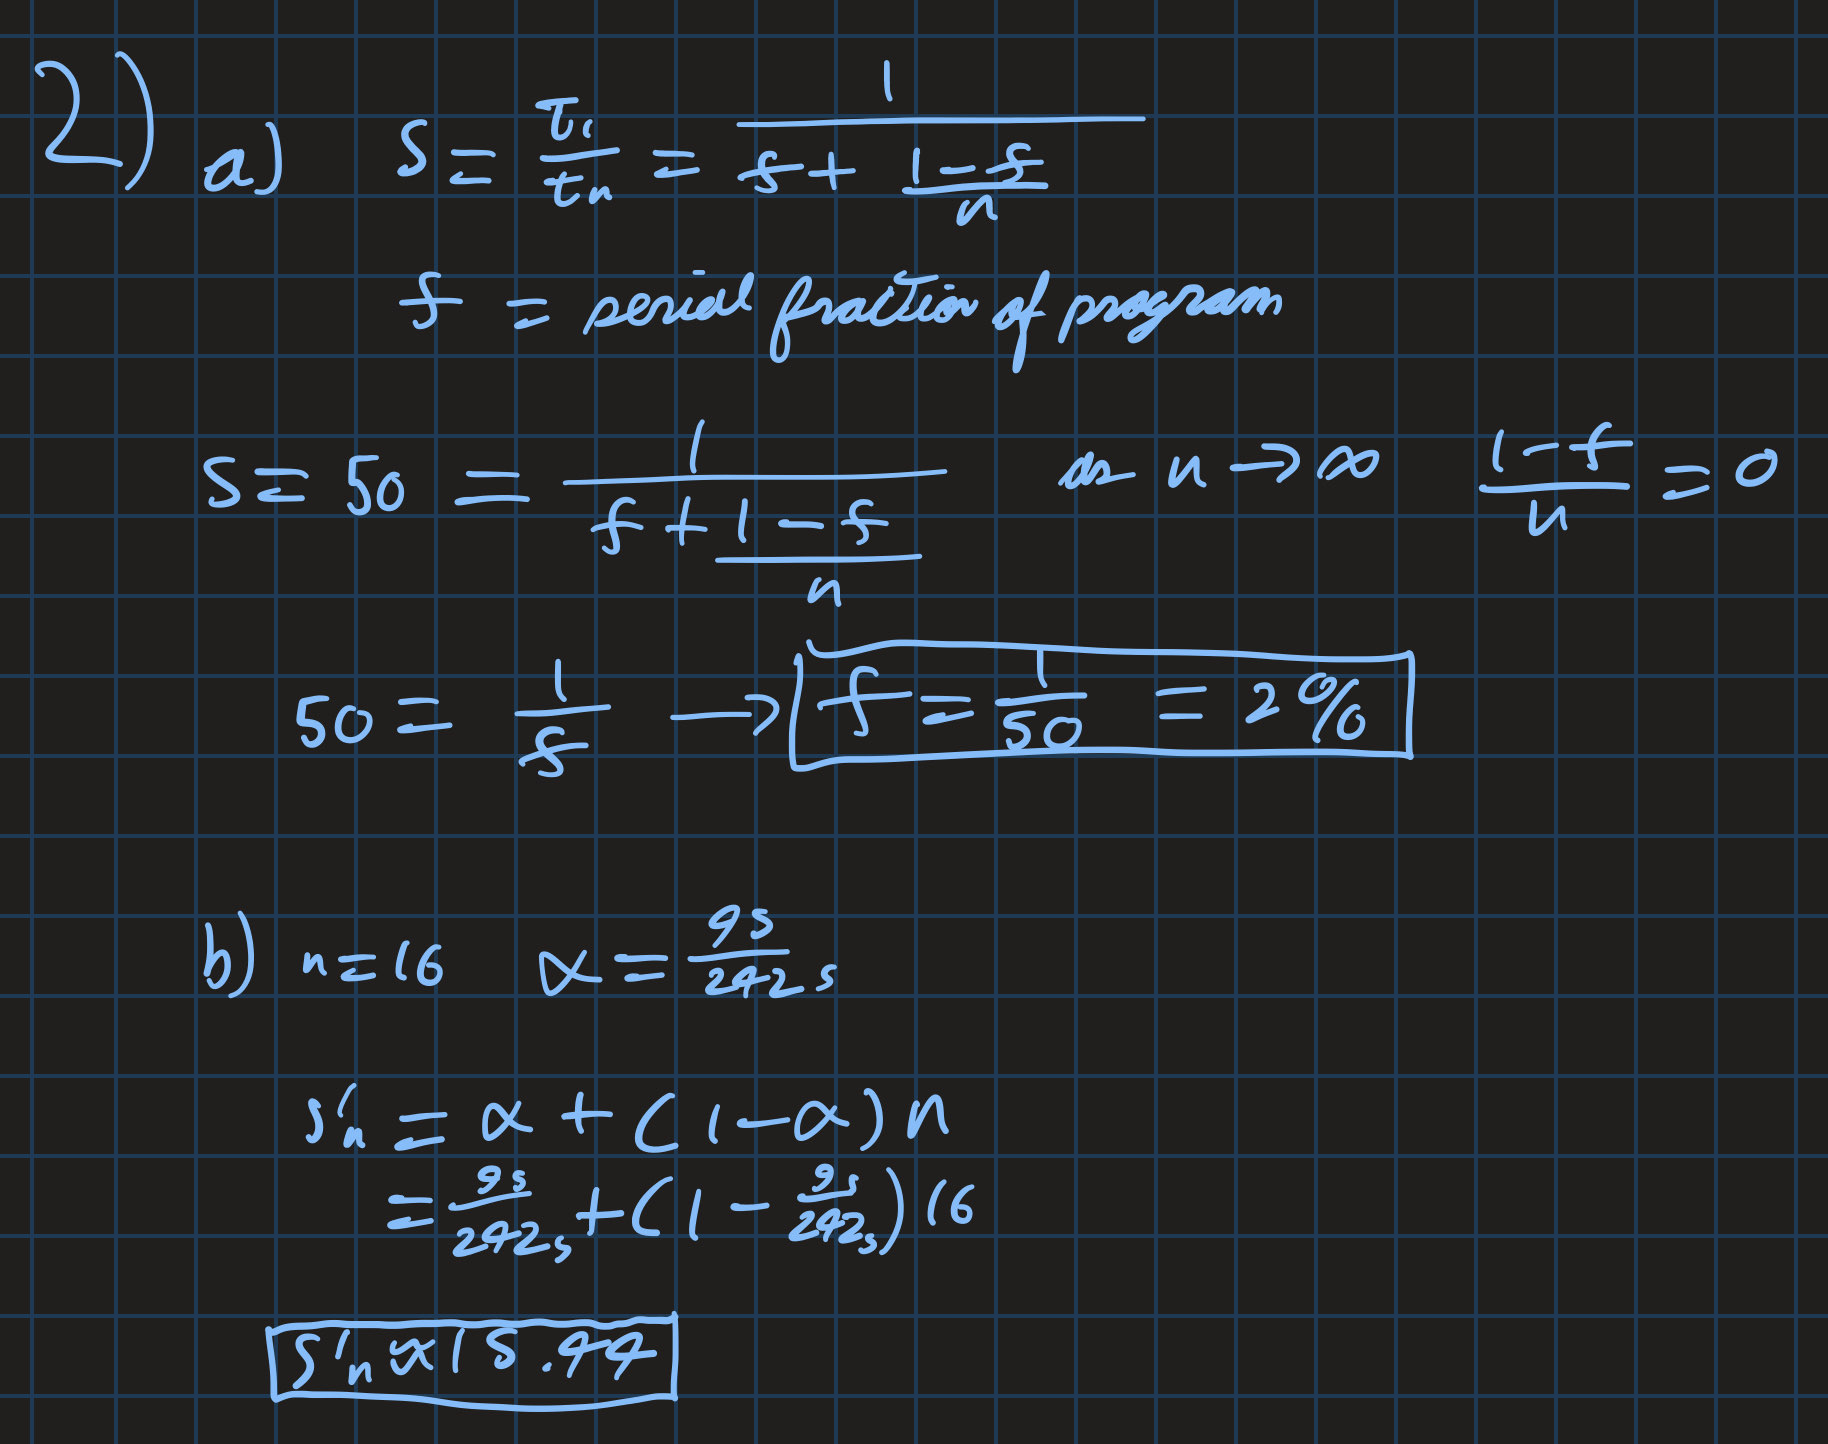
\includegraphics[width=0.9\textwidth]{./images/q2.jpg}
\caption{Math for Question 2}
\label{fig:q2}
\end{figure}

\newpage

\section*{Q3:}

% \begin{figure}[H]
% \centering
%     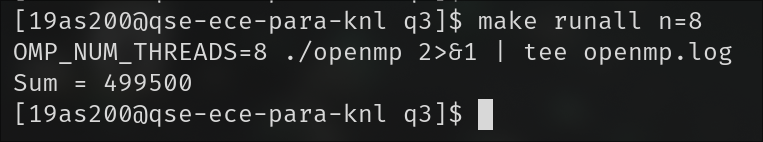
\includegraphics[width=0.9\textwidth]{./images/q3.jpg}
% \caption{Math for Question 3}
% \label{fig:q3}
% \end{figure}

\newpage

\section*{Q4:}

\begin{figure}[H]
\centering
    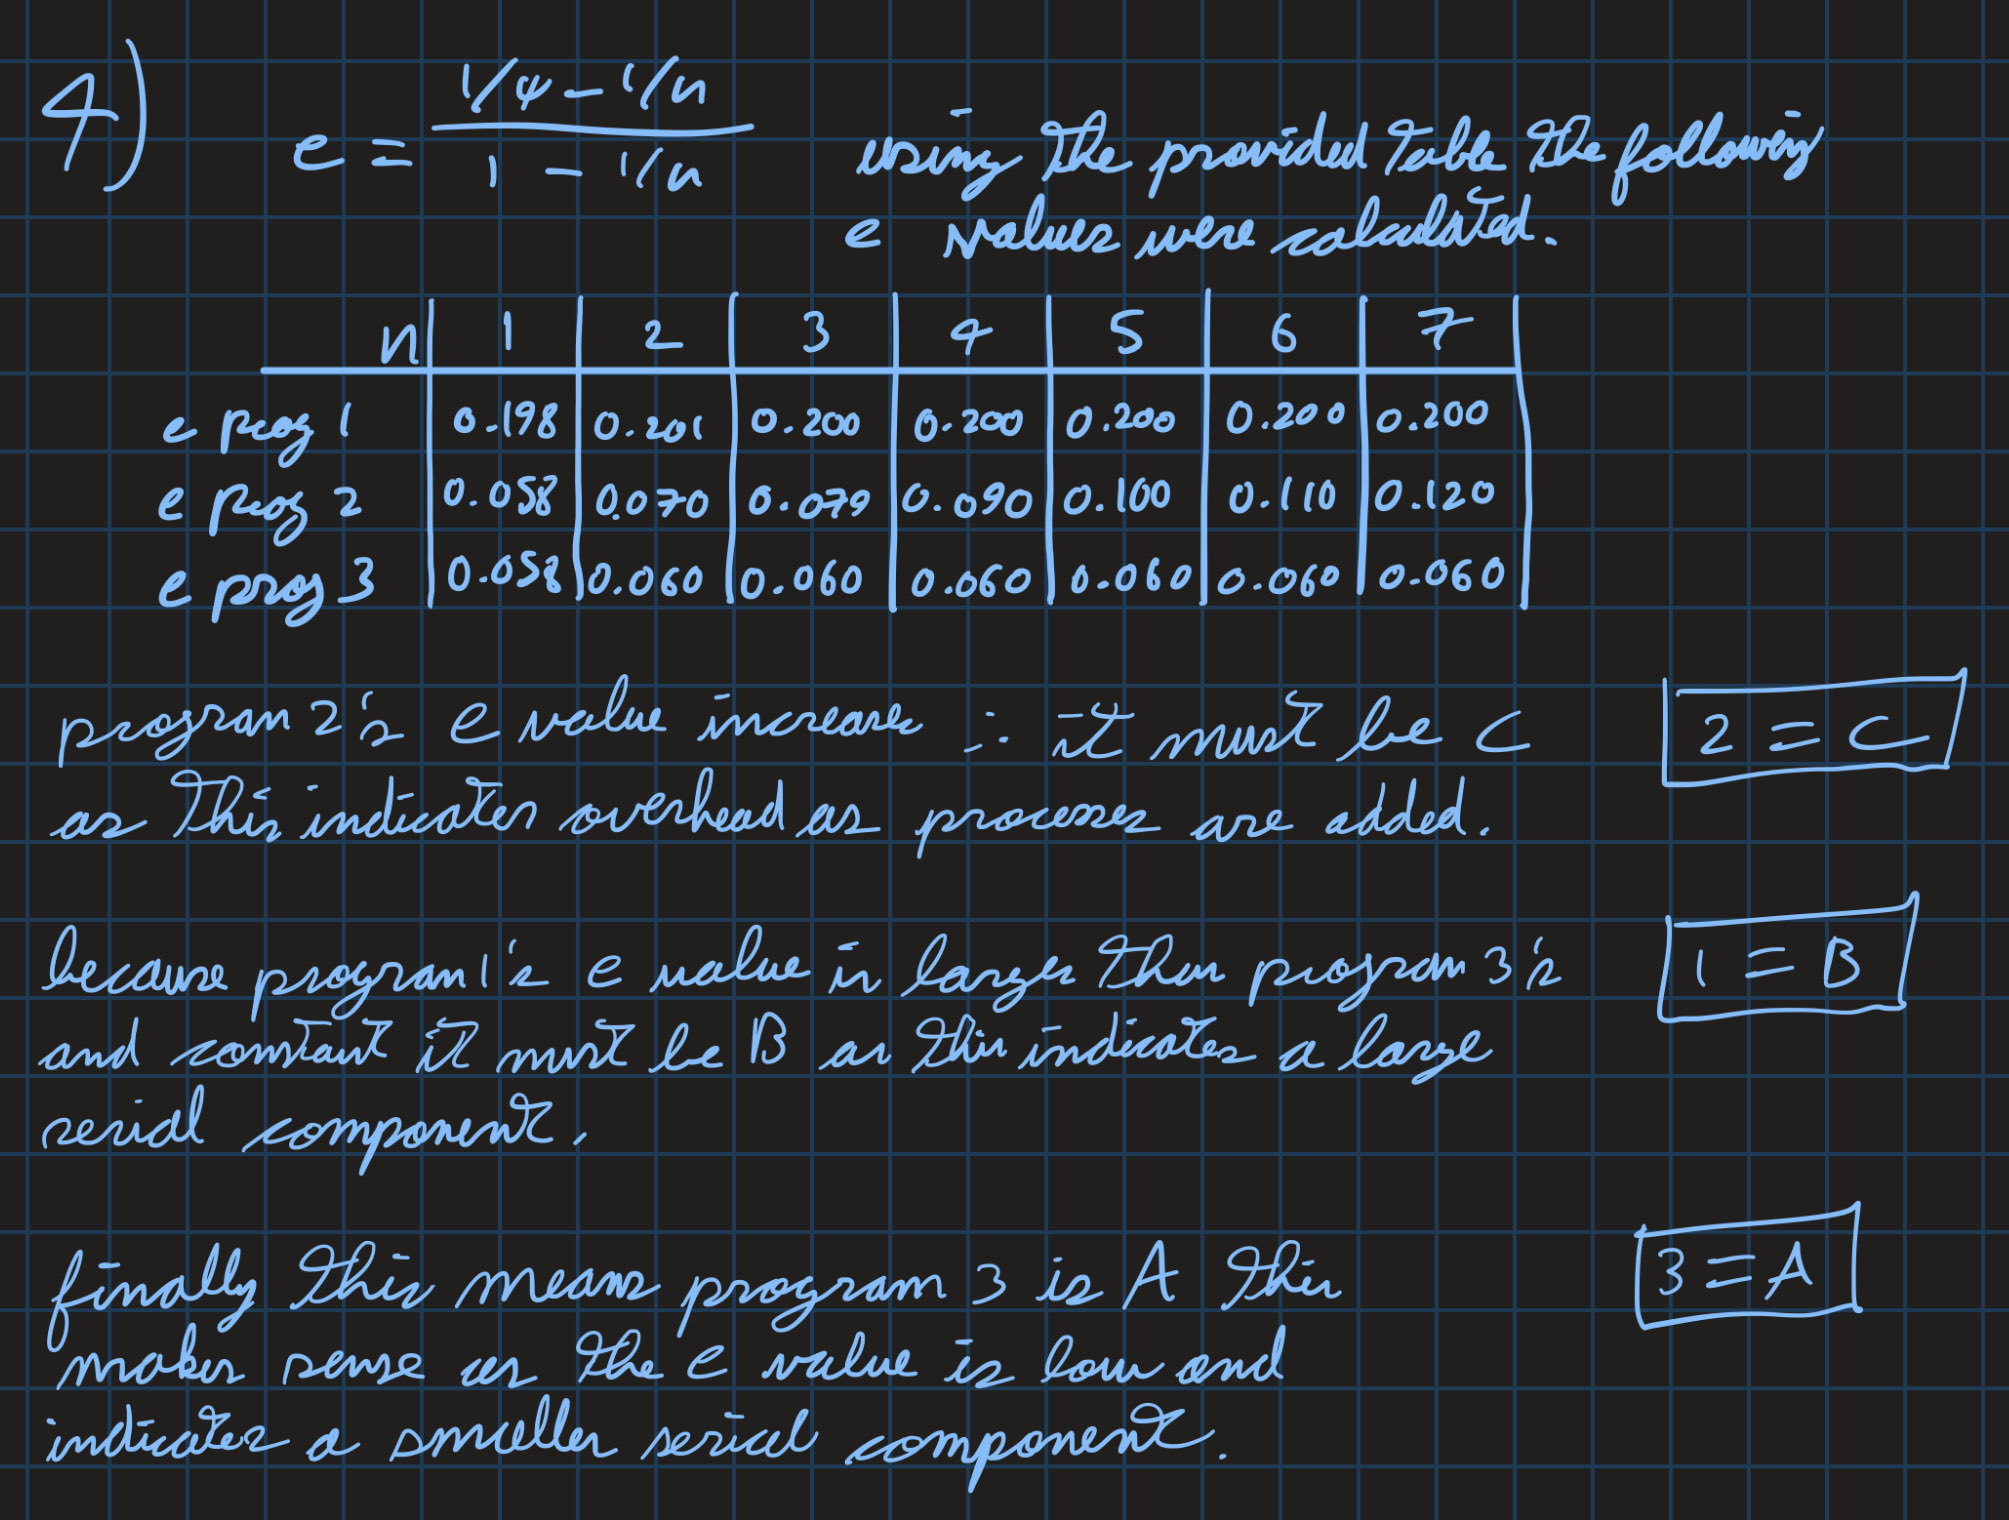
\includegraphics[width=0.9\textwidth]{./images/q4.jpg}
\caption{Math for Question 4}
\label{fig:q4}
\end{figure}

\newpage

\section*{Q5:}

\begin{figure}[H]
\centering
    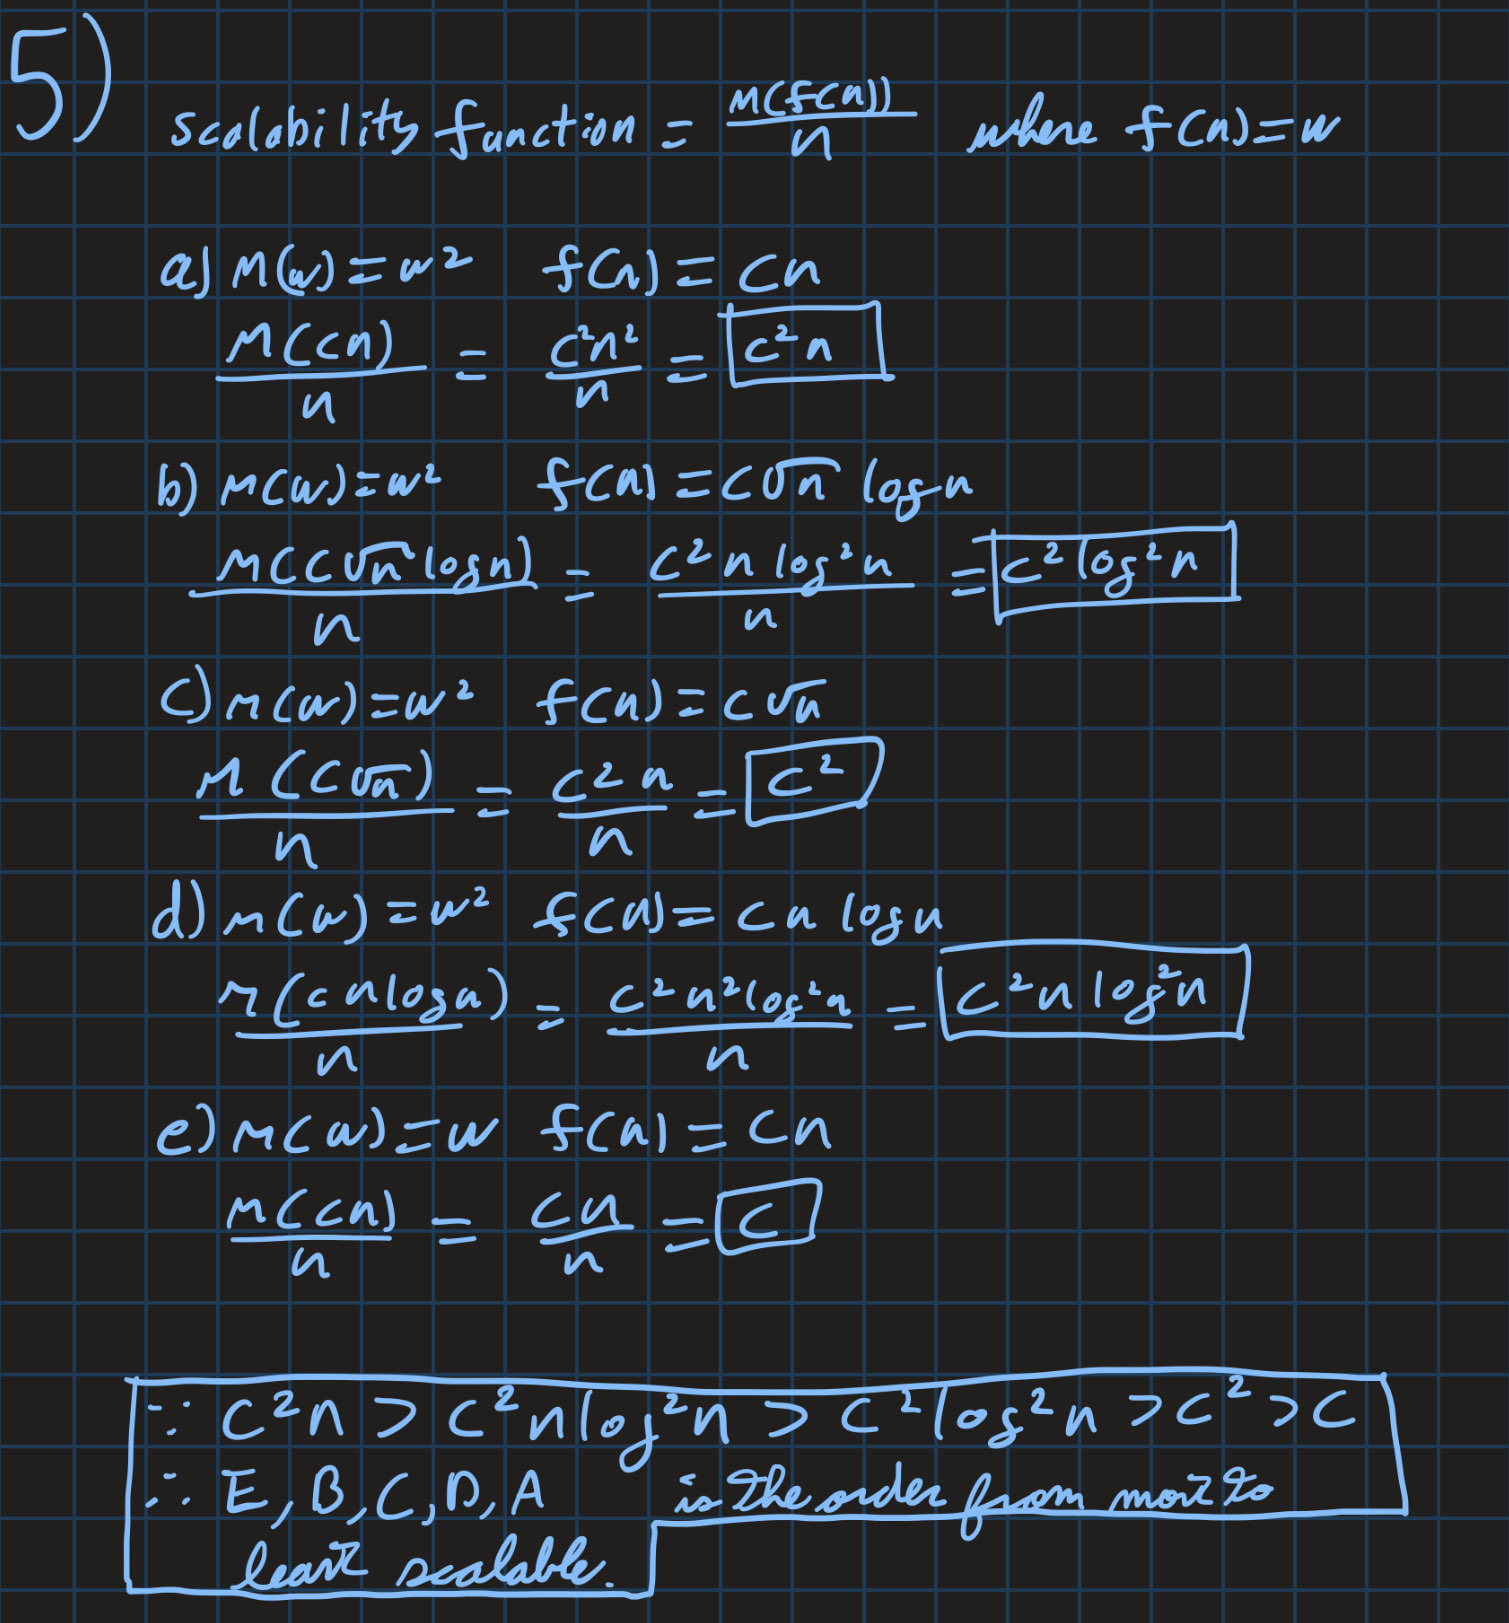
\includegraphics[width=0.9\textwidth]{./images/q5.jpg}
\caption{Math for Question 5}
\label{fig:q5}
\end{figure}

\newpage

\section*{Q6:}

\begin{figure}[H]
\centering
    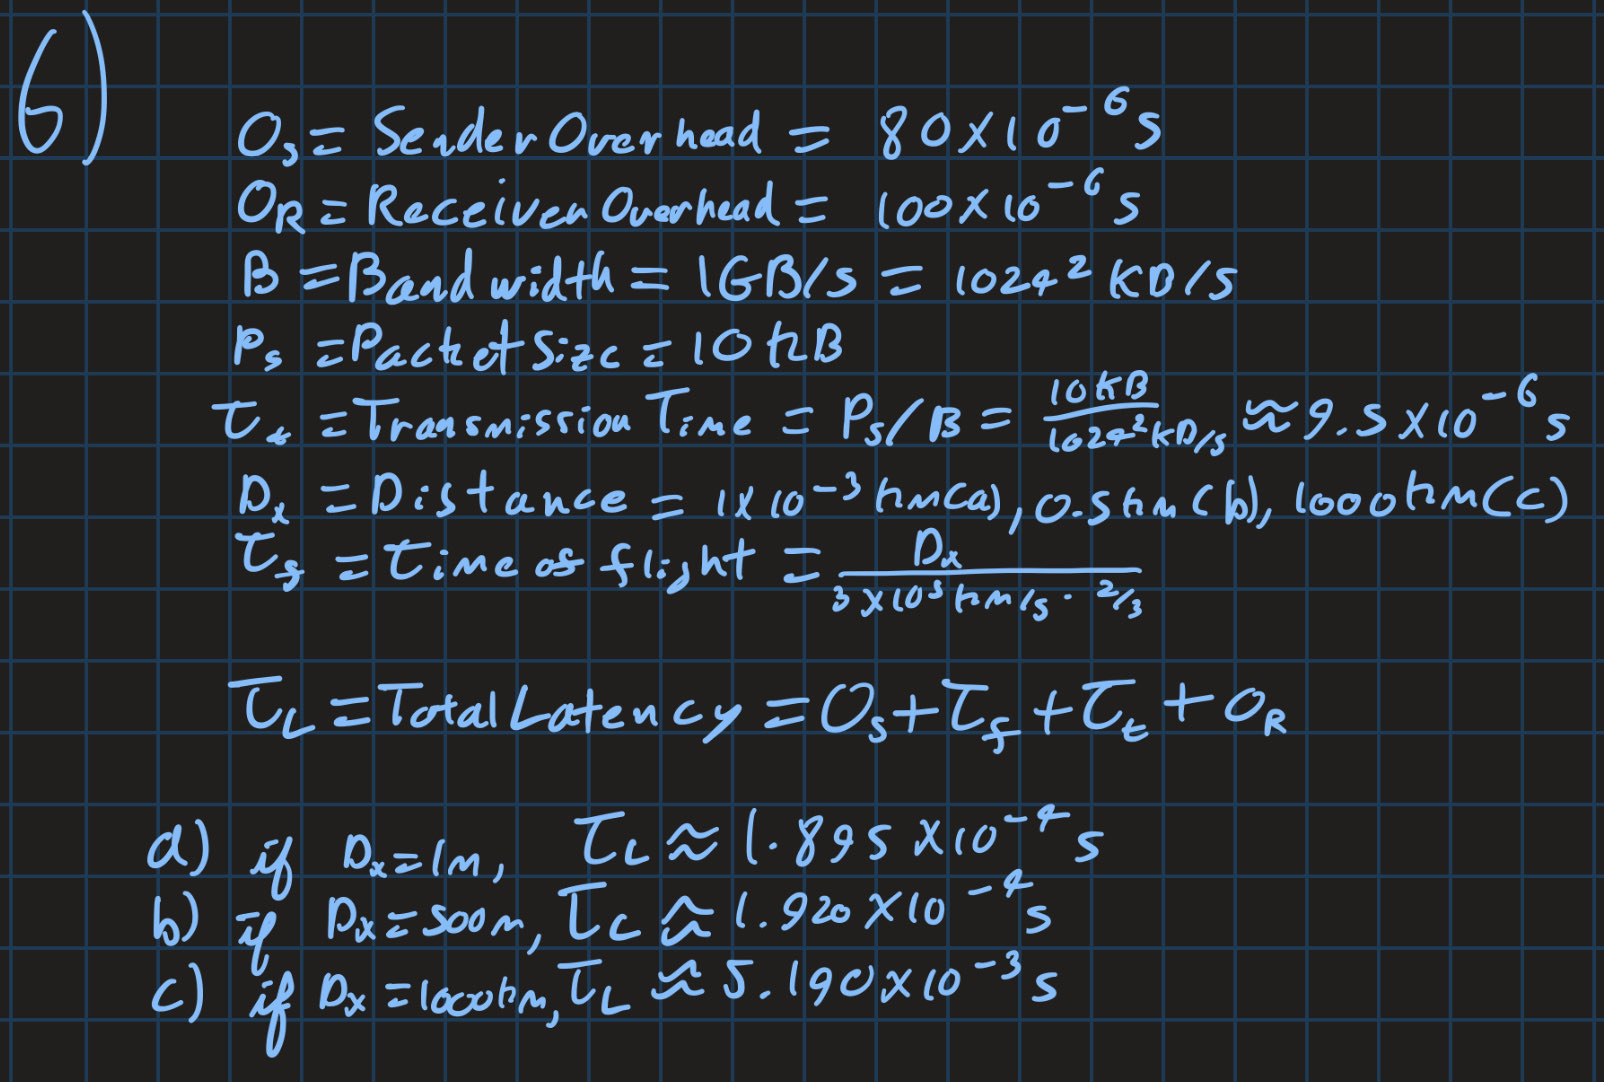
\includegraphics[width=0.9\textwidth]{./images/q6.jpg}
\caption{Math for Question 6}
\label{fig:q6}
\end{figure}

\newpage


\section*{Q7:}

\begin{figure}[H]
\centering
    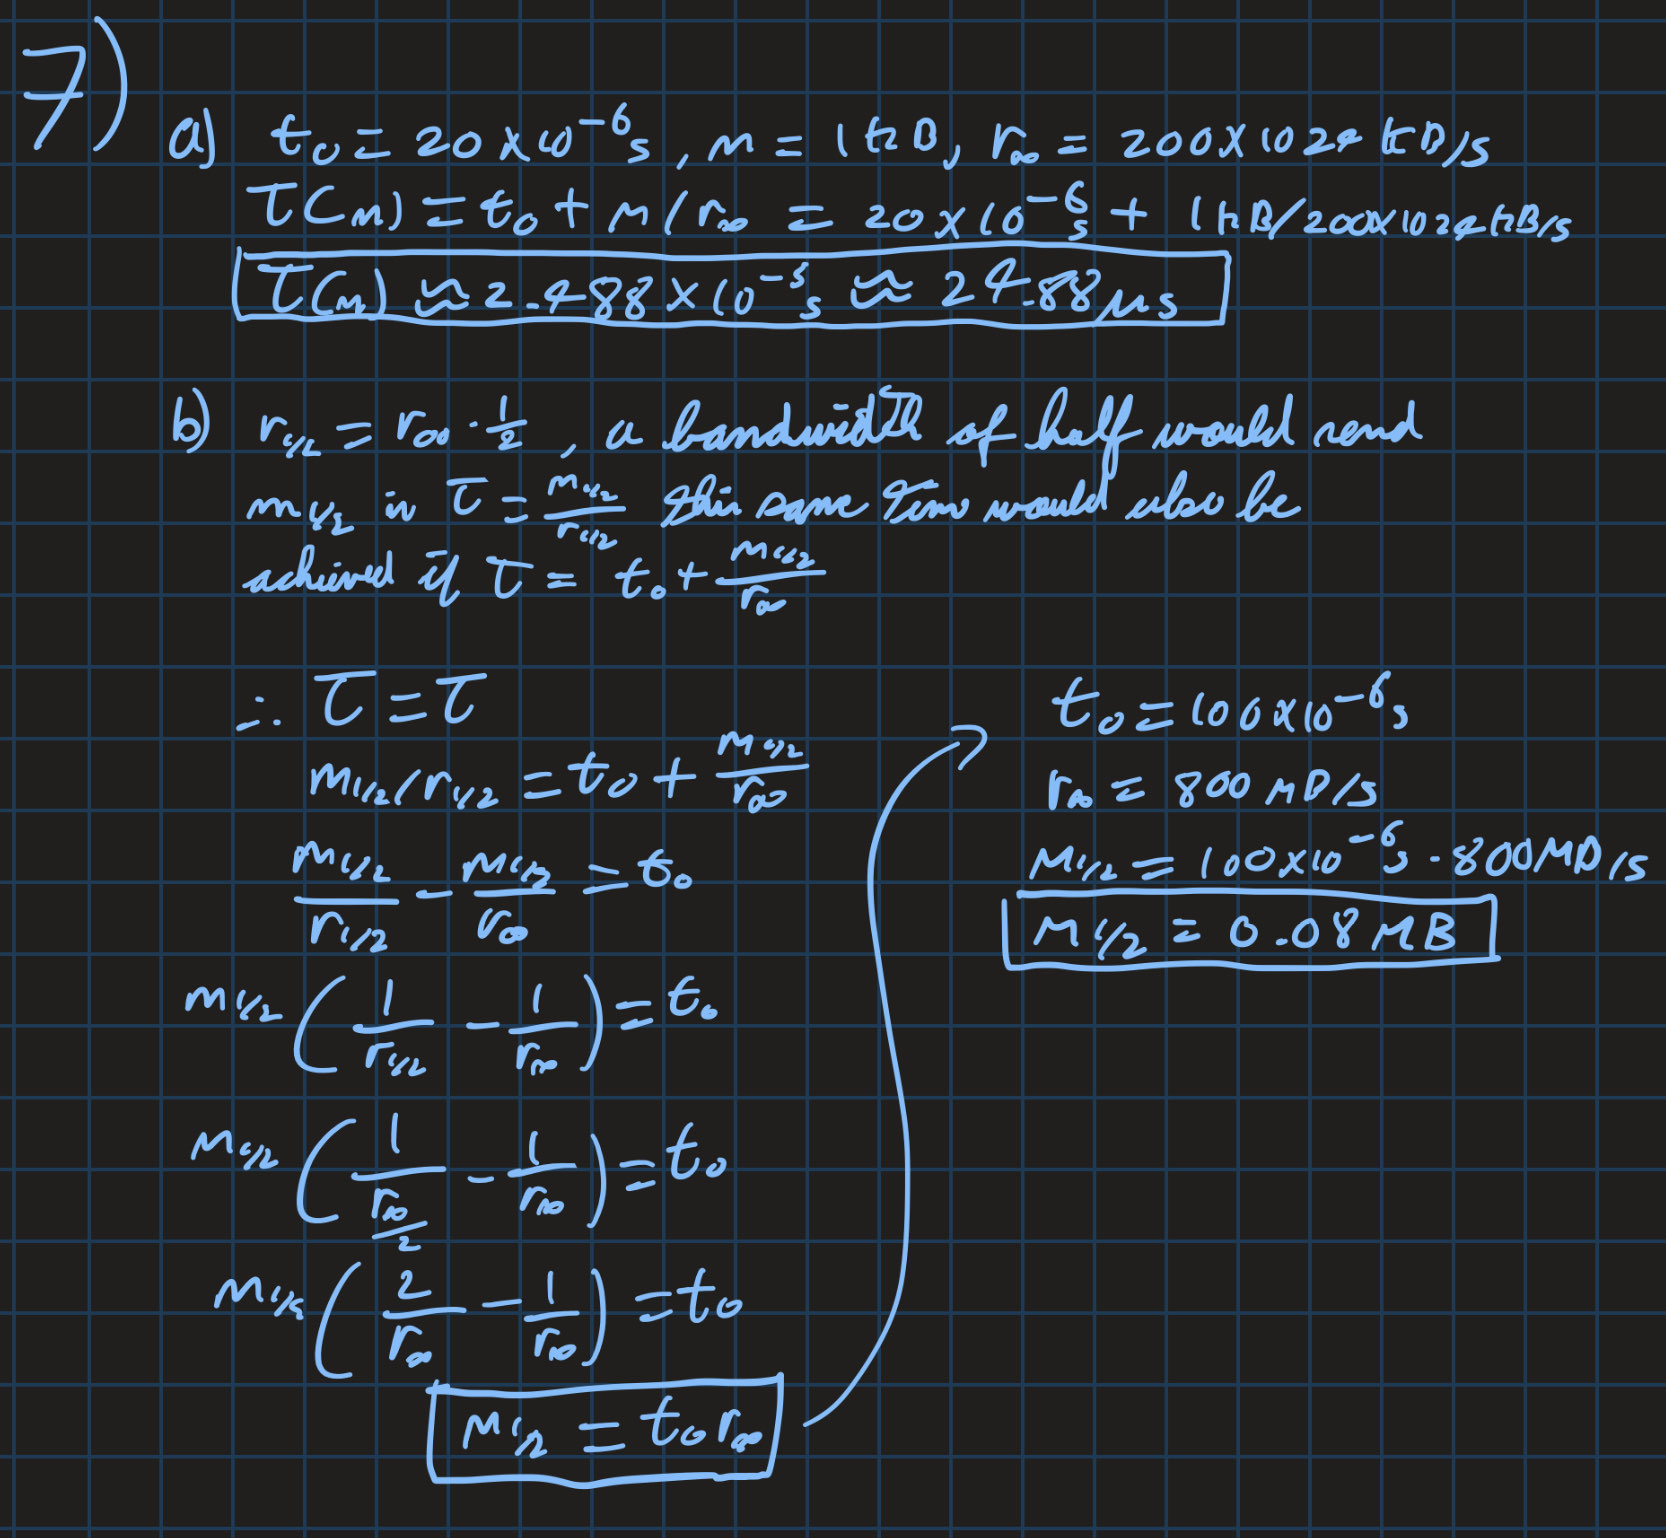
\includegraphics[width=0.9\textwidth]{./images/q7.jpg}
\caption{Math for Question 7}
\label{fig:q7}
\end{figure}

\newpage

\section*{Q8:}
\newpage

\section*{Q9:}
\lstinputlisting[language=C, caption=\centering{MPI code for question 9}, label={q9:mpi}]{../q9/mpi.c}
\newpage

\section*{Q10:}
\lstinputlisting[language=C, caption=\centering{MPI code for question 10}, label={q10:mpi}]{../q10/mpi.c}
\newpage

\begin{appendices}\label{Appendix}
\end{appendices}

\end{document}
